\begin{figure}[!htbp]
  \centering
  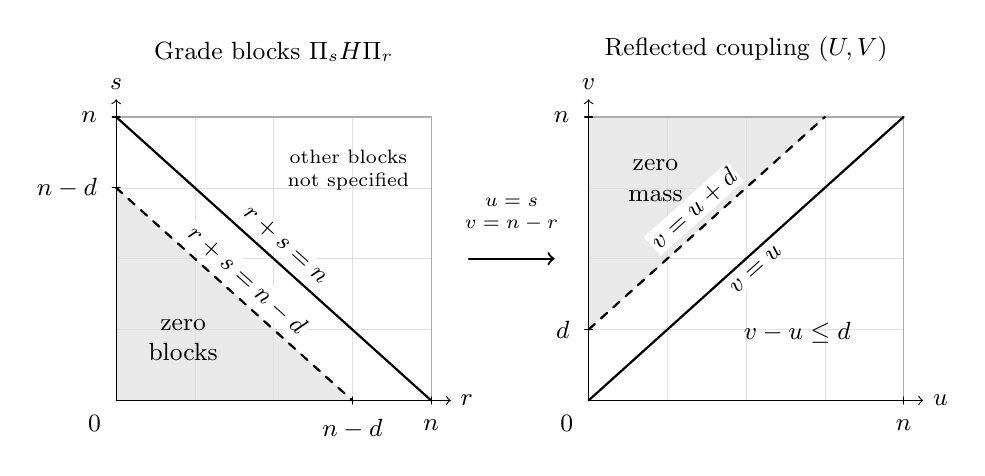
\begin{tikzpicture}[x=1cm,y=.9cm,line cap=round,line join=round,
                      font=\small]
    \begin{scope}
      \fill[gray!17] (0,0) -- (3,0) -- (0,3) -- cycle;
      \draw[step=1,gray!25,very thin] (0,0) grid (4,4);
      \draw[gray!65] (0,4) -- (4,4) -- (4,0);
      \draw[->] (0,0) -- (4.25,0) node[right] {$r$};
      \draw[->] (0,0) -- (0,4.25) node[above] {$s$};
      \node[below left=2pt] at (0,0) {$0$};
      \draw (3,.05) -- (3,-.05) node[below=2pt] {$n-d$};
      \draw (4,.05) -- (4,-.05) node[below=2pt] {$n$};
      \draw (.05,3) -- (-.05,3) node[left=2pt] {$n-d$};
      \draw (.05,4) -- (-.05,4) node[left=2pt] {$n$};
      \draw[thick,dashed] (0,3) -- (3,0)
        node[midway,above=2pt,sloped,fill=white,inner sep=1pt]
        {$r+s=n-d$};
      \draw[thick] (0,4) -- (4,0)
        node[midway,above=2pt,sloped,fill=white,inner sep=1pt]
        {$r+s=n$};
      \node[align=center] at (.85,.85) {zero\\blocks};
      \node[align=center,font=\scriptsize] at (2.95,3.25)
        {other blocks\\not specified};
      \node[above=10pt] at (2,4.25) {Grade blocks $\Pi_sH\Pi_r$};
    \end{scope}

    \draw[->,thick] (4.48,2) -- (5.57,2);
    \node[align=center,font=\scriptsize] at (5.02,2.63)
      {$u=s$\\$v=n-r$};

    \begin{scope}[xshift=6cm]
      \fill[gray!17] (0,1) -- (0,4) -- (3,4) -- cycle;
      \draw[step=1,gray!25,very thin] (0,0) grid (4,4);
      \draw[gray!65] (0,4) -- (4,4) -- (4,0);
      \draw[->] (0,0) -- (4.25,0) node[right] {$u$};
      \draw[->] (0,0) -- (0,4.25) node[above] {$v$};
      \node[below left=2pt] at (0,0) {$0$};
      \draw (4,.05) -- (4,-.05) node[below=2pt] {$n$};
      \draw (.05,1) -- (-.05,1) node[left=2pt] {$d$};
      \draw (.05,4) -- (-.05,4) node[left=2pt] {$n$};
      \draw[thick,dashed] (0,1) -- (3,4)
        node[midway,above=2pt,sloped,fill=white,inner sep=1pt]
        {$v=u+d$};
      \draw[thick] (0,0) -- (4,4)
        node[midway,below=2pt,sloped,fill=white,inner sep=1pt]
        {$v=u$};
      \node[align=center] at (.85,3.1) {zero\\mass};
      \node at (2.65,.95) {$v-u\le d$};
      \node[above=10pt] at (2,4.25) {Reflected coupling $(U,V)$};
    \end{scope}
  \end{tikzpicture}
  \[
    \mathbb P\{R=r,S=s\}
      =2^{-n}\|\Pi_sH\Pi_r\|_{\mathrm{HS}}^2,
    \qquad r+s-n=u-v.
  \]
  \caption{Grade blocks and their reflected coupling, schematic for $0<d<n$.
  Under $U=S$, $V=n-R$, the zero-block region $r+s<n-d$ becomes the
  zero-mass region $v-u>d$, giving $V-U\le d$ almost surely.
  Dashed boundaries are allowed; solid diagonals mark $r+s-n=u-v=0$.
  Each marginal is $\operatorname{Bin}(n,1/2)$. Unshaded locations need
  not carry positive mass, and grid spacing is illustrative.}
  \label{fig:grade-coupling}
\end{figure}
